% \documentclass[handout]{beamer}
\documentclass{beamer}

\mode<presentation>
{
  \usetheme{ANLBlue}
  % \usefonttheme[onlymath]{serif}
  % \usetheme{Singapore}
  % \usetheme{Warsaw}
  % \usetheme{Malmoe}
  % \useinnertheme{circles}
  % \useoutertheme{infolines}
  % \useinnertheme{rounded}

  \setbeamercovered{transparent=20}
}

\usepackage[english]{babel}
\usepackage[latin1]{inputenc}
\usepackage{alltt,listings,multirow,ulem,siunitx}
\usepackage[absolute,overlay]{textpos}
\TPGrid{1}{1}
\usepackage{pdfpages}
\usepackage{ulem}
\usepackage{multimedia}
\usepackage{multicol}
\newcommand\hmmax{0}
\newcommand\bmmax{0}
\usepackage{bm}
\usepackage{comment}
\usepackage{subcaption}

% font definitions, try \usepackage{ae} instead of the following
% three lines if you don't like this look
\usepackage{mathptmx}
\usepackage[scaled=.90]{helvet}
% \usepackage{courier}
\usepackage[T1]{fontenc}
\usepackage{tikz}
\usetikzlibrary{decorations.pathreplacing}
\usetikzlibrary{shadows,arrows,shapes.misc,shapes.arrows,shapes.multipart,arrows,decorations.pathmorphing,backgrounds,positioning,fit,petri,calc,shadows,chains,matrix,mindmap}

\newcommand\vvec{\bm v}
\newcommand\bvec{\bm b}
\newcommand\bxk{\bvec_0 \times \kappa_0 \cdot \nabla}
\newcommand\delp{\nabla_\perp}

% \usepackage{pgfpages}
% \pgfpagesuselayout{4 on 1}[a4paper,landscape,border shrink=5mm]

\usepackage{JedMacros}

\newcommand{\timeR}{t_{\mathrm{R}}}
\newcommand{\timeW}{t_{\mathrm{W}}}
\newcommand{\mglevel}{\ensuremath{\ell}}
\newcommand{\mglevelcp}{\ensuremath{\mglevel_{\mathrm{cp}}}}
\newcommand{\mglevelcoarse}{\ensuremath{\mglevel_{\mathrm{coarse}}}}
\newcommand{\mglevelfine}{\ensuremath{\mglevel_{\mathrm{fine}}}}

%solution and residual
\newcommand{\vx}{\ensuremath{x}}
\newcommand{\vc}{\ensuremath{\hat{x}}}
\newcommand{\vr}{\ensuremath{r}}
\newcommand{\vb}{\ensuremath{b}}

%operators
\newcommand{\vA}{\ensuremath{A}}
\newcommand{\vP}{\ensuremath{I_H^h}}
\newcommand{\vS}{\ensuremath{S}}
\newcommand{\vR}{\ensuremath{I_h^H}}
\newcommand{\vI}{\ensuremath{\hat I_h^H}}
\newcommand{\vV}{\ensuremath{\mathbf{V}}}
\newcommand{\vF}{\ensuremath{F}}
\newcommand{\vtau}{\ensuremath{\mathbf{\tau}}}


\title{Practical Multigrid Methods \\ for Momentum Balance in Ice Sheets}
\subtitle{This talk: \url{http://59A2.org/files/20150202-LIWGMultigrid.pdf}}

\author{{\bf Jed Brown} \texttt{jed@jedbrown.org} (ANL and CU Boulder)}

% - Use the \inst command only if there are several affiliations.
% - Keep it simple, no one is interested in your street address.
% \institute
% {
%   Mathematics and Computer Science Division \\ Argonne National Laboratory
% }

\date{Land Ice Working Group, NCAR, 2015-02-02}

% This is only inserted into the PDF information catalog. Can be left
% out.
\subject{Talks}


% If you have a file called "university-logo-filename.xxx", where xxx
% is a graphic format that can be processed by latex or pdflatex,
% resp., then you can add a logo as follows:

% \pgfdeclareimage[height=0.5cm]{university-logo}{university-logo-filename}
% \logo{\pgfuseimage{university-logo}}



% Delete this, if you do not want the table of contents to pop up at
% the beginning of each subsection:
% \AtBeginSubsection[]
% {
% \begin{frame}<beamer>
%   \frametitle{Outline}
%   \tableofcontents[currentsection,currentsubsection]
% \end{frame}
% }

\AtBeginSection[]
{
  \begin{frame}<beamer>
    \frametitle{Outline}
    \tableofcontents[currentsection]
  \end{frame}
}

% If you wish to uncover everything in a step-wise fashion, uncomment
% the following command:

% \beamerdefaultoverlayspecification{<+->}

\begin{document}
\lstset{language=C}
\normalem

\begin{frame}
  \titlepage
\end{frame}

\begin{frame}{Why do we need scalable solvers?}
  \begin{itemize}
  \item Increasing resolution
    \begin{itemize}
    \item larger problem sizes
    \item more 3D effects visible
    \item more time steps $\implies$ smaller budget per time step
    \end{itemize}
  \item Sequence of simulations -- data assimilation, UQ
  \item All other costs typically linear in problem size
  \end{itemize}
\end{frame}

\begin{frame}
  \includegraphics[width=\textwidth]{figures/KeyesStrongWeak} \\
  \uncover<2>{\large \alert{The easiest way to make software scalable is to make it sequentially inefficient. -- Gropp 1999}}
\end{frame}

\begin{frame}{Is multigrid needed?}
  \begin{itemize}
  \item Long-range coupling is slow to converge using local methods
    \begin{itemize}
    \item Iteration count proportional to diameter of support of Green's functions
    \end{itemize}
  \item How local are the Green's functions?
    \begin{itemize}
    \item Columns of the inverse matrix
      \begin{equation*}
        u(x) = \int_{y \in \Omega} G(x,y) f(y)
      \end{equation*}
    \item Sticky, flat bad -- Green's functions local (and SIA is accurate)
    \item Slippery bed (ice shelf), steep topography at high resolution
    \item Pressure: surface is Dirichlet boundary condition, causes rapid decay
    \end{itemize}
  \end{itemize}
\end{frame}

\input{slides/GroundingLine/Steepness.tex}
\begin{frame}[shrink=5]{Hydrostatic equations for ice sheet flow}
  \begin{itemize}
  \item Valid when $w_x \ll u_z$, independent of basal friction {\small (Schoof\&Hindmarsh 2010)}
  \item Eliminate $p$ and $w$ from Stokes by incompressibility:\\
    \quad 3D elliptic system for $\bm u = (u,v)$
    \begin{align*}
      - \nabla\cdot \left[ \eta
        \begin{pmatrix}
          4 u_x + 2 v_y & u_y + v_x & u_z \\
          u_y + v_x & 2 u_x + 4 v_y & v_z
        \end{pmatrix} \right] + \rho g \bar\nabla h & = 0
    \end{align*}
    \begin{align*}
      \eta(\theta,\gamma) &= \frac{B(\theta)}{2} (\gamma_0 + \gamma)^{\frac{1-n}{2n}}, \qquad n \approx 3 \\
      \gamma &= u_x^2 + v_y^2 + u_xv_y + \frac 1 4 (u_y+v_x)^2 + \frac 1 4 u_z^2 + \frac 1 4 v_z^2
    \end{align*}
    and slip boundary $\sigma \cdot \bm n = \beta^2 \bm u$ where
    \begin{align*}
      \beta^2(\gamma_b) &= \beta_0^2 (\epsilon_b^2 + \gamma_b)^{\frac{m-1}{2}}, \qquad 0 < m \le 1 \\
      \gamma_b &= \frac 1 2 (u^2 + v^2)
    \end{align*}
  \item $Q_1$ FEM with Newton-Krylov-Multigrid solver in PETSc: \code{src/snes/examples/tutorials/ex48.c}
  \end{itemize}
\end{frame}

\input{slides/THI/Y5kmClip.tex}
\begin{frame}
  \begin{figure}
    \includegraphics[width=\textwidth]{figures/THI/y-10km-m10p6l5-ew}
    \centering\caption{Grid sequenced Newton-Krylov convergence for test $Y$.
    The ``cliff'' has \SI{58}{\degree} angle in the red line ($12\times 125$ meter elements), \SI{73}{\degree} for the cyan line ($6\times 62$ meter elements).}\label{fig:testy}
  \end{figure}
\end{frame}
\input{slides/THI/Shaheen.tex}
\begin{frame}
  \begin{center}
    \alert{\huge One high-accuracy solve \\[0.2em]
      costs 30 times as much \\[0.5em]
      as a residual evaluation}
  \end{center}
  \begin{center}
    about 15 to reach truncation error

    \bigskip

    \uncover<2>{\alert{\large 1000 times faster than some popular methods} \\
      e.g. Lemieux, Price, Evans, Knoll, Salinger, Holland, Payne 2011 \\ (J. Computational Physics) \\
      --- Actual speedup subject to Amdahl's Law}
    
    \bigskip

    {(Brown, Smith, Ahmadia 2013, SIAM J. Scientific Computing)}
  \end{center}
\end{frame}
\begin{frame}{Algebraic multigrid for Hydrostatic}
  \begin{itemize}
  \item Easy to use: assemble a matrix and throw it over the wall
  \item Higher setup costs, lower arithmetic intensity
  \item AMG uses heuristics to diagnose anisotropy; varies by discretization
  \item Need to represent rotational modes
    \begin{itemize}
    \item Smoothed aggregation takes a ``near null space'' (translation plus rotation)
    \end{itemize}
  \end{itemize}
\end{frame}
\input{slides/HydrostaticEigen.tex}

\begin{frame}{HPGMG-FE \quad \url{https://hpgmg.org}}
  \centering 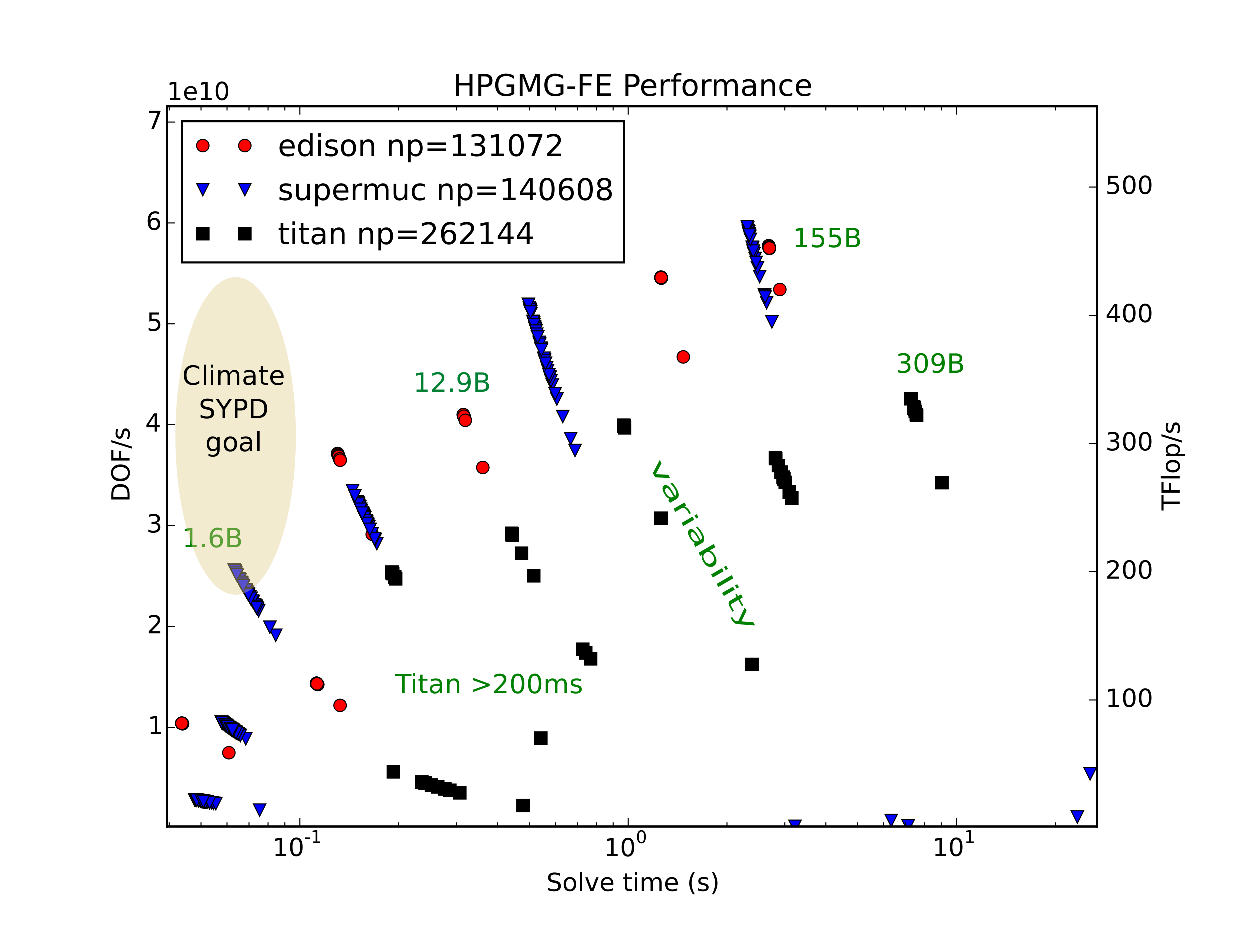
\includegraphics[width=.9\textwidth]{figures/hpgmg/range-edison-supermuc-titan-ann2}
\end{frame}


\newcommand\smallterm[1]{{\color{gray} #1}}
\begin{frame}{Conservative (non-Boussinesq) two-phase ice flow}
  Find momentum density $\rho\uu$, pressure $p$, and total energy density $E$:
  \begin{gather*}
    (\rho\uu)_t + \div (\smallterm{\rho\uu\otimes\uu} - \eta D\uu_i + p\bm 1) - \rho \bm g = 0 \\
    \rho_t + \div \rho\uu = 0 \\
    E_t + \div \big((E+p)\uu - k_T\nabla T - k_\omega\nabla\omega \big) - \eta D\uu_i\tcolon D\uu_i - \smallterm{\rho\uu\cdot\bm g} = 0
  \end{gather*}
\begin{itemize}
\item Solve for density $\rho$, ice velocity $\uu_i$, temperature $T$, and melt fraction $\omega$ using constitutive relations.
\item This and many other formulations lead to a Stokes problem
\end{itemize}
\end{frame}

\input{slides/MonolithicOrSplit.tex}
\input{slides/Stokes/WeakFormNewtonStep.tex}

\input{slides/HardwareArithmeticIntensity.tex}

\begin{frame}{Outlook}
  \begin{itemize}
  \item Choose suitable technology
  \item Geometric multigrid is simple and has low setup cost
  \item Algebraic multigrid has higher setup, more finicky to discover anisotropy
  \item Stokes problems
    \begin{itemize}
    \item block factorization is easiest (all run-time options in PETSc)
    \item coupled MG is worth considering
    \end{itemize}
  \item Newton linearization of sliding
  \item Mind the external factors
  \end{itemize}
\end{frame}

\end{document}
